%%% 3Background / %%%
\chapter{Background} \label{ch:background}
To understand the interpretation of interaction graph and design of endorsement
model, basic concepts about graph properties and metrics is required.
Similarly, Blockchain relies a lot on cryptographic functions to maintain its
property of the secure, immutable and attack-resilient structure. This chapter,
therefore, provides a general overview of the background concepts that is
required for the subsequent sections. 
%This chapter provides an overview of the basic concepts necessary to understand
%the subsequent sections.

\section{Graph properties}
A graph, as the name suggests can be used to represent objects and their
relationships graphically. \\
Formally, a graph~\cite{bondy1976graph}, G, is an ordered triple
\displaystyle{(V,E,$\varphi _G$)} where, \\
\displaystyle{V} \text{ is a non empty set of vertices } \displaystyle{ v}.
\\ \displaystyle{E} \text{ is a non empty set of edges } \displaystyle{ e}.
\\ \displaystyle{e} \text{ connects two vertices, where, } \displaystyle{v
\in V } \text{ and } \displaystyle{e \in E}. \\ \displaystyle{\varphi _G}
\text{ is an incidence function that assigns pair of vertices to each edge
of the graph G.} \\ \displaystyle{\varphi _G(e) = uv} \text{ represents
that } \displaystyle{e} \text{ is an edge that joins vertices }
\displaystyle{u} \text{ and } \displaystyle{v} \\

Based on these properties, any online interaction system can be modeled
graphically including reputation system. Each node on the network can represent
agents/users that interact with other users. This interaction can represent the
relationship between nodes as the edges connecting vertices. The transfer of
data between the nodes can be quantified to represent the weight of the edge.
This weight value can be used to determine the strength or weakness of
relationship between the nodes. Modeling the interaction as a graph can help
to understand and analyze its complexity at different level. By observing the
local properties of a particular node such as its activity, connection degree,
its neighbors, and interactions, one can derive useful information about a node.
Similarly, the node's relative position in a given graph can help to determine
its centrality and connectivity. An overall structure of the network(graph
topology) can help to study the global properties of the graph. 

Network metrics that are helpful in analyzing the complexity of interactions at
different levels~\cite{gkorou2014exploiting} and used for evaluation of results
in this project are: \\
\textbf{Degree Connectivity:} The number of connections a node has is the
degree of its connectivity. The number of inflow is referred to as indegree
whereas the number of outflows is the outdegree of a node. Usually, a higher
degree of connectivity implies a higher likelihood for information(relevant
data to the network) to pass through that node.\\
\textbf{Network Centrality:} Centrality refers to the significance of a node in
the network. i.e., how important the node is in the overall network. The degree
of connectivity is one way to measure centrality of a node. Similarly, there
are other centrality measures which includes: Closeness centrality,
Betweenness centrality, Prestige centrality.\\ 
\textbf{Closeness centrality} refers to how close a node is to other nodes in
the network.  \\
\textbf{Betweenness centrality} refers to the number of nodes to
which the given node acts as a connector. i.e., how many nodes passes through
this node.\\
\textbf{Prestige centrality} refers to the significance of the node
based on the significance of the adjacent nodes(nodes one is connected to).  To
observe and analyze the behavior at the macro-level, one needs to look at the
overall structure of the graph. i.e., Network topology that shows how
constituent parts are interconnected to form the graph as a whole. They can
form ring, star, tree, or mesh structure or be a fully connected graph where
each node are connected to each other. 
%cite graph theories and applications:
%http://citeseerx.ist.psu.edu/viewdoc/download?doi=10.1.1.721.3161&rep=rep1&type=pdf
%more concept based on what is needed to know when representing/modeling the network.

%\subsection{EigenTrust}
%EigenTrust is a reputation management algorithm for P2P network that aims to minimize 
%malicious behaviour in the network and is based on the notion of transitive trust.
%i.e. If a peer \textit{i} trusts a peer \textit{j} then all other peers trusted by 
%\textit{j} is also trusted by \textit{i}. 
%In EigenTrust, global reputation of each peer \textit{i} is given by local trust value 
%assigned to peer \textit{i} by other peers and is weighted by the global reputation 
%of assigning peers. 
%A local trust value $s_{ij}$ is calculated by 
%each peer \textit{i} which represents the opinion \textit{i} has of \textit{j}. $s_{ij}$
%is the difference of satisfactory and unsatisfactory transactions peer \textit{i} had 
%with other peers \textit{j}.
%\begin{equation}
%	s_{ij} = sat(i,j) - unsat(i,j) \\ 
%\end{equation}
%where sat(i,j) represents number of satisfactory transactions that \textit{i} had with 
%\textit{j} whereas unsat(i,j) represents number of unsatisfactory transactions. \\
%To prevent malicious peers from assigning arbitrarily high local trust values to 
%other malicious peers, the local trust value is normalized as $c_{ij}$ before aggregating 
%them. 
%\begin{equation}
%	c_{ij} = \frac{max(s_{ij},0)}{\sum_{j}max(s_{ij},0)}
%\end{equation}
%$C_{ij}$ keeps changing depending on the good or bad interaction between peer \textit{i} 
%and peer \textit{j}.
%Based on the local trust value assigned by other peers, each peer has a global trust 
%value that determines their standing in the network. To aggregate the normalized local 
%trust values, the approach used is friend-friend reference where a peer \textit{i} 
%would ask its acquaintances about their opinion about other peers. Trust that 
%peer \textit{i} places in peer \textit{k} by asking his friends can be denoted by 
%$t_{ik}$ as : 
%\begin{equation}
%	t_{ik} = \sum_{j} c_{ij} c_{jk}
%\end{equation}
%Each peer asks other peers about their opinion which is weighted based on how much peer 
%\textit{i} trusts them. 
%If we define C as a matrix $[c_{ij}]$ and $t_{i}$ as a vector containing values 
%$t_{ik}$, then $t_{ik}$ = $C^T\vec{c_{i}}$. This helps a peer get a wider view of 
%the network more than its own experience. This can continue for many nodes until peer 
%\textit{i} asks his friend's friend's and friend's friend can be consulted further to 
%receive a broader view of the network. For \textit{n} nodes, we can represent \textit{t}
%as t = $(C^T)^n c_{i}$. For a large enough value of \textit{n} , trust vector 
%$\vec{t_{i}}$ will converge to same vector for every peer \textit{i} and could give 
%complete view of the network. 
%\textit{t} is the global trust vector where $t_{j}$ quantifies the trust system places in 
%peer \textit{j}. 
%EigenTrust is robust to malicious peers and good for decreasing inauthentic file downloads 
%in a P2P network. However, it doesn't address the issues such as inactive peers, where a 
%peer doesn't download from anywhere else, malicious collectiveness, where malicious peers 
%collude to inflate the trust value. It also doesn't have a way to calculate negative trust 
%and is entirely based on user feedback. ~\cite{kamvar2003eigentrust}
%
% The approach used for deriving these 
% values are past history and friend-friend reference. 

%cite: http://ilpubs.stanford.edu:8090/562/1/2002-56.pdf
%cite: https://www.cs.indiana.edu/~kapadia/courses/I590-Fall-09/internal/eigentrust.pdf

%\subsection{Net flow Rate convergence}
%Net flow rate convergence can help to determine anomaly in the network. By looking at how 
%fast the net flow converges to zero, it can detect unusual behaviour in the network. 
%The flow in a network can be measured by looking at inflow and outflow edges and 
%calculating their differences. Inflow edges are all incoming edges in the graph and 
%outflow edges are all outgoing edges . (diagram) Net flow convergence rate is the rate at which the net flow converges to the global net flow which is zero. 
%Depending upon how fast the net flow in a graph converges to zero, it can be useful to 
%detect anomaly.(example diagram) 
%
%cite: Decentralized Reputation system for transaction network. 
%Net flow convergence is used by (cite) and seems useful in detecting sybil node. 

%\subsection{Binomial Random Walk}

\section{Cryptography} \label{sec:cryptography}
\subsection{Basic Concepts}
Cryptography offers algorithms to achieve confidentiality, integrity,
authenticity, and non-repudiation. Confidentiality and integrity ensure that
the information being communicated is not disclosed or has been modified to or
by any unauthorized parties. The data is hidden/encrypted such that only the
authorized parties can make sense out of it. i.e., decrypt using the previously
agreed upon key. Authenticity relates to confirming the truth of an attribute
claimed by an entity. Non-repudiation is associated with the property that any
entity who has previously sent the message cannot deny their
authorship~\cite{katz1996handbook}. \\ 
A cryptosystem can be defined as a five-tuple $\displaystyle(P, C, K, E, D)$ where, 
\begin{itemize}
	\item $\displaystyle P, \text{ is a finite set of plain texts. }$
	\item $\displaystyle C, \text{ is a finite set of ciphertexts. } $
	\item $\displaystyle E,$ \text{ set of encryption rules such that}
		$\displaystyle e_{k}:P \Rightarrow C$
	\item $\displaystyle D,$ \text{ set of decryption rules such that}
		$\displaystyle d_{k}:C  \Rightarrow P$ 
	\item For each k $\displaystyle \in$ K, there is $\displaystyle e_k \in E$
		and $\displaystyle d_k \in D$ such that $\displaystyle d_k(e_k(m)) = m$
		for every plaintext $\displaystyle m \in P$
\end{itemize}
%$\displaystyle P$, is a finite set of plaintexts and $\displaystyle C$, a finite set of ciphertexts. \\
%E, set of encryption rules such that $e_{k}:P \Rightarrow C $. \\ 
%D, set of decryption rules such that $d_{k}:C \Rightarrow P$\\ 
%For each k in $in$ K, there is $e_{k } \in$E and $d_{k } \in$ D such that
%$d_{k}(e_{k}(m))$= m for every plaintext m $\in$ P.\\

A cryptosystem can be either symmetric or asymmetric. Symmetric makes use of
the same key for both encryption and decryption whereas asymmetric, also known
as public-key cryptography makes use of key pairs, public and private keys. The
public key can be publicly distributed, and an entity 'A' wishing to send a
confidential message to other entity 'B' can encrypt the message using B's
public key $k_{p}$ to form ciphertext c. Upon receiving c, B can decrypt it
using the private key $k_{s}$ that is only known to B and corresponds to the
respective public key that was used to form c. The computation of $k_{s}$ given
$k_{p}$ is computationally infeasible in a secure system. Besides public-key
encryption, public-key cryptography also has use in digital signature as
discussed in section~\ref{ss:digitalsignature}. RSA~\cite{rivest1978method} is
one example of a public-private cryptosystem.

% A cryptosystem shouldn't rely on the privacy of algorithm used to secure the system. 
% According to Kerckhoff's principle, a cryptosystem should be secure even if everything 
% about the system, except the key, is public knowledge. Another encryption method 
% known as public key cryptography makes use of two different keys for encryption 
% and decryption respectively. It uses public key and private key pairs that are related 
% but is hard to deduce one from the other. When sending a message, one might make public 
% the public key to the whole network but the private key must not be known/shared with 
% anyone but the owner himself. 
%Diffie-Hellman key exchange
%encryption, decryption 

\subsection{Hash functions}
Cryptographic hash functions are one-way functions, also known as mathematical
trapdoor function that transforms an input message into a fixed length binary
output. It is one way because although converting a message input to a hash
value or a message digest can be done in constant time, reversing the operation
is practically impossible to achieve as it is computationally inefficient. An
important characteristics of hash function is its deterministic output. i.e.,
given an input, it will always produce the same output. This attribute
contributes to data verifiability as anyone can always verify if the produced
hash output for data matches by simply applying the data to the respective hash
function. 
Other significant properties of hash function that contributes to
reliability in digital security are~\cite{mironov2005hash}: \\
One-way: Given a key k, and an output w, it should be hard for an attacker to find x
such that the hash of x applied with k, produces w. ie., $H_k(x)$ = w.\\ 
Second pre-image resistant: Given a key k and a string x, it should be hard for
an attacker to find y such that $H_k(x)$ = $H_k(y)$.\\ 
Collision-resistant: Given a key k, it should be hard for an attacker to find x and y such that
$H_k(x)$ = $H_k(y)$. \\
Earlier hash functions include MD5 which produced an output of size 128 bits.
Collision-resistant attack in MD5 is possible within seconds with a complexity
of $2^{39}$~\cite{wang2005break} MD5 operations. NIST published secure hashing algorithm (SHA)
in 1993 as the secure hash standard. Currently, SHA-3 is the latest in SHA
family of standards that was released in 2015 with SHA-0, SHA-1 and SHA-2 as
it's predecessor algorithms. Collision attack for SHA-1 was shown to be
practically pssible~\cite{stevens2017first} by creating two colliding pdf files
that produced same SHA-1 digest. It took equivalent processing power of 6,500
years of single CPU computation time and 110 years of GPU computation time.
Applications of hashing algorithms include digital signature, ISO checksums,
fingerprinting data etc. This cryptographic hash functions is relevant for
understanding blockchain data structure. Especially significant for
verification of transactions that make use of hash tree, namely Merkle Tree for
including list of transactions in the block and chaining the blocks together.
\begin{figure}
	\begin{center}
		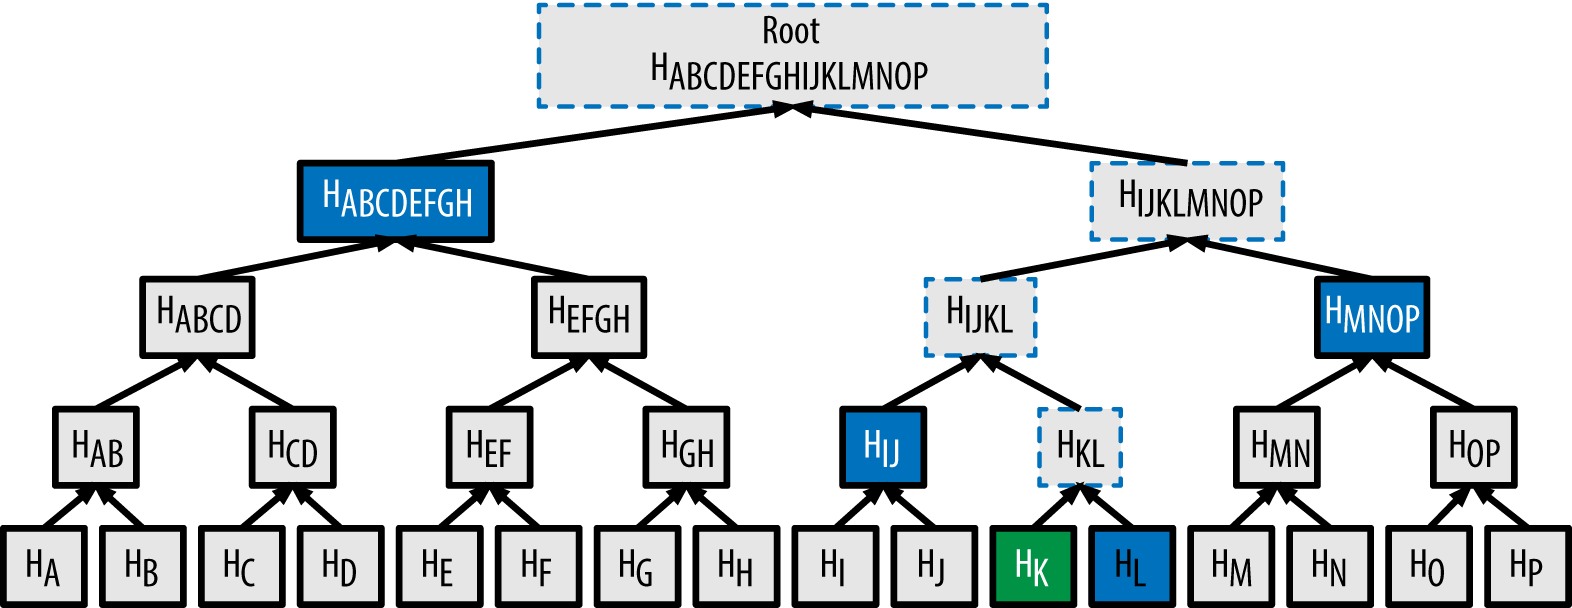
\includegraphics[width=0.8\textwidth]{Images/MerkleeTree.eps}
		\caption{Merkle Tree}
		\label{fig:merkleTree}
	\end{center}
\end{figure}
To create merkle tree, list of transactions are paired and hashed together.
This process is repeated until there is only one hash value left which acts a
root value of the tree. This root hash is included as a block header that
entails all the transactions data. Figure ~\ref{fig:merkleTree} illustrates the
process of creating a merkle root. 
Two significant use of merkle tree are: \\
\begin{enumerate}
	\item Data integrity verification: An attempt to change any transaction data
		would completely change the root hash of the block.  
	\item Data inclusion verifcation: It is easy to verify the inclusion of a
		transaction in a block without requiring to include all the
		transactions. From figure ~\ref{fig:merkleTree}, to verify inclusion of
		transaction $H_{K}$, only the hash values that are shown in blue needs to
		stored.  \\
\end{enumerate}

The PoW consensus mechanism, relies on SHA-256 hash(in Bitcoin)
applied to the block header and nonce to produce a verifiable fingerprint of
data. This is discussed in more detail in ~\ref{sec:blockchain}. Proof-of-work
was originally used in 1997 by Adam Back as a anti-spam system for the then
proposed Hashcash~\cite{back2002hashcash}. The general idea being that the
sender of message would have to compute some number of sha operations before
sending the message.  The generated fingerprint could be checked by anyone to
see if the sender has actually done the required number of computations. If a
legitimate user sending out one email had to spend 'x' seconds to do the sha
operations, a malicious user intending to send thousands of emails had to spend
1000x seconds. \\



%Cryptographic hash functions are a one-way function, also known as mathematical
%trapdoor function that transforms an input message into a fixed length binary
%output. It is one way because although converting a message input to a hash
%value or a message digest can be done in constant time, reversing the operation
%is practically impossible to achieve as its computationally inefficient.
%Earlier hash functions include MD5 which produces a 128-bit hash value but is
%vulnerable and can be cracked by brute force attack.  The predecessors hash
%functions are sha-256 preceeded by sha-1, sha-2 and others. Their applications
%include the digital signature, message authentication both of which are
%interesting for blockchain as will be discussed in section(name). The essential
%characteristics of hash functions are their deterministic output, meaning given
%a fixed input; it will always generate the same output. It offers collision
%resistant property, i.e. it is impossible or extremely rare to get the same
%hash value for two different messages.  If m1 and m2 are the message and h(m1)
%and h(m2) are hash functions applied to them respectively, collision resistant
%ensures that h(m1) != h(m2). Another important characteristic of a hash
%function is that the hash value does not indicate the original information that
%was hashed thus making it efficient for hiding information.
%
%deterministic output 
%computationally efficient
%hash collision: collision resistant h(m1) != h(m2)
%hide information
%sha-1, sha-2, sha-256 

\subsection{Digital Signature} \label{ss:digitalsignature}
A digital signature acts as an intermediary to prove that an entity A, has the
password without ever requiring A to reveal it. As discussed earlier,
public-key cryptography uses key-pairs that correspond with each other. In
context of Blockchain, If Alice wants to send a value(transaction) to Bob, she
can create a transaction message, sign it using her private key and broadcast
the transaction over the network. Her signature and the transaction message
will be publicly available on the network(assuming a public blockchain
network). Anyone on the network can verify that the signature corresponds to
Alice's public key. Thus, Alice can always prove that she is the owner of the
public key from where the message originated. The signature is dependent on the
message, and therefore any attempt to modify the message will refute the
signature.

%figure showing basic process

\section{Blockchain Technology} \label{sec:blockchain}
Blockchain Technology is a variant of distributed database implemented on a P2P
network. Every participating node in the network has the same copy of history
of records of database. Blockchain is essentially a chain of blocks, as the
name suggests. Each block consists of list of valid transactions(signed
messages) collected by validators/miners of the network. The linking and
ordering of transactions are also the responsibility of validators. The
validators proposes a block they have unlocked to the network which can either
be accepted or rejected. If accepted, the newly created block gets linked to
the existing blockchain with a hash pointer pointing to the previous block. As
such, blockchain provides the transaction ordering that every node agreed on at
a given time. Consensus metric helps to establish and maintain the integrity of
a blockchain
system\footnote{https://github.com/ethereumbook/ethereumbook/blob/develop/consensus.asciidoc}.
The primary attributes that constitute a blockchain system are distributed,
decentralized, time-stamped transactions.  
There have been P2P protocols deployed as a file-sharing or other form of
content delivery services before Blockchain. What separates Blockchain from
them is that for the first time, it made possible to transfer values online on
a P2P network without a double-spending problem. i.e., If a peer 'A' sends a
file or a value 'v' to 'B,' then the file should be owned by 'B' and removed
from the account of A. 'A' should not be able to send the same file 'v' to
other entities on the network. This was the significant contribution of the
technology. 
%While, transferring digital contents, sharing information were
%possible before, transferring values was made possible by Blockchain
%technology.

%~\cite{pilkington201611}

%\subsection{Basic Concepts}
%transaction, message, signature, broadcast, verify, network, miners, validate, write blocks 

\subsection{Evolution \& Categories}
Bitcoin was the first application that made use of Blockchain technology which
was a peer-to-peer electronic cash system. The major contribution of this
application was solving distributed trust at scale without using a trusted
intermediary. 
Along the dimension of validation and access control~\cite{voronchenko2017you},
blockchains can be categorized as a public permissionless system, public
permissioned, and private permissioned. 
\begin{itemize}
	\item Public Permissionless:Anyone can join the network and become a writer
		of the block as long as they can solve a problem or reach the consensus
		that satisfies the underlying protocol. The records are publicly
		available and thus publicly verifiable. 
	\item Public Permissioned: Anyone can still join the network, but a writer
		of the block is known but not necessarily trusted entity. The records
		are publicly verifiable. 
	\item Private Permissioned: This is similar to a Public permissioned
		setting, but the records are not made public and therefore doesn't
		offer public verifiability. This kind of setup is more specific to
		business use-cases where one business doesn't need to know about other
		business policies or customer information etc. 
\end{itemize}
~\cite{voronchenko2017you} provides a detailed discussion on various blockchain
types and their uses.


\subsection{Consensus Mechanisms}
As a distributed database with multiple writers, there has to be a way for
everyone to reach a consensus on a shared global view of the network. Consensus
mechanisms allow doing so. Based on consensus mechanisms, systems can be
distinctly categorized into\footnote{Categorization based on Hashgraph's presentation \cite{baird2016hashgraph}}:
\begin{itemize}
	\item Leader Based System: In this case, there is a pre-selected leader
		that collects all the transactions and appends new records to the
		blockchain. Having a small group or consortium, it has low
		computational requirements. As a blockchain protocol, it offers an
		immutable audit of the records. However, just like any other
		centralized system, this system is susceptible to DDOS attacks and
		third-party(leader) interference. Generally used in a private or
		permissioned blockchain setup, it offers higher throughput compared to
		public permissionless blockchains. Examples include Hyperledger Fabric,
		R3 Corda etc. 
	\item Proof-Of-Work: This is the most widely used consensus mechanism in a
		public permissionless setup. As the name suggests, a validator/miner
		needs to provide the proof to the network that it has done a
		significant amount of work. This work requires miners to invest a
		substantial amount of computational resource. The reason for this is
		that everyone(all miners) compete to be the writer of the next block
		for which they need to solve a cryptographic puzzle. Mainly, they need
		to find a hash value that can be associated with the proposed block.
		The only way to find this value is by brute-forcing.  The simplified
		overview of this mining process is given by figure
		~\ref{fig:cryptographicPuzzle} 
		\begin{figure}
			\begin{center}
			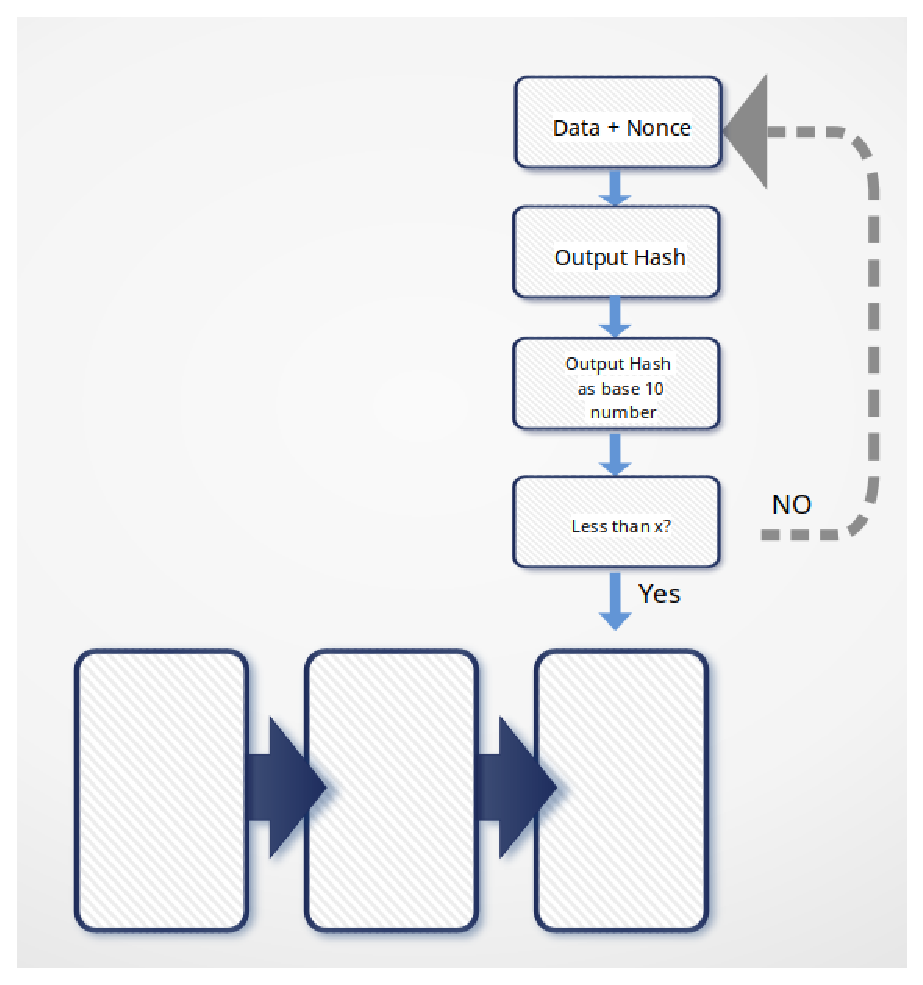
\includegraphics[width=0.5\textwidth]{Images/CryptographicPuzzle.eps}
			\caption{Cryptographic Puzzle}
			\label{fig:cryptographicPuzzle}
			\end{center}
		\end{figure}
		The apparent advantage of such consensus mechanism is that it makes the
		system DDOS resistant while offering immutable audit trail and
		scalability.  However, miners can still decide upon the order of
		transactions to include in the block although they cannot modify the
		transaction. As such, one could term this as 'unfair' since the
		transaction doesn't get picked up in order of when it was broadcasted
		to the network. 
	\item Economy based systems: Consensus mechanisms such as Proof-of-stake or
		delegated proof-of-stake can be seen as an economy based system. Unlike
		PoW, miners don't compete with each other to be the writer of next
		block thus saving lots of computational resources. The general idea is
		that participants can put the respective platform based native token
		they own at stake to validate a block. Whoever has the highest value at
		stake gets to write the next block. If the participation turned out to
		be a malicious one, then all the tokens that were at stake get lost. As
		such, it puts scarce resource at stake. However, this includes problem
		such as nothing-at-stake~\cite{houy2014will}. i.e., a node could vouch for two forks
		of the same blockchain with nothing to lose. Other drawbacks of this
		approach are that there is no certainty of consensus, and often has no
		total ordering of transactions. Examples include Casper etc. 
\end{itemize}

\subsection{Smart contracts}
A contract in a classical sense is a set of rules with pre-defined obligations
and permissions that participants are assumed to follow. 
A smart contract, however is a computer program that can codify the
interaction between participating entities and self-executes when triggered by
an event. It doesn't necessarily need to be legally binding or even associated
with the outside world~\footnote{https://universe.ida.dk/media/23422289/fritz-henglein.pdf}.
The term Smart contact was first coined by Cryptographer Nick Szabo, in 1994
~\cite{SzaboSmart1994} and defined as a computerized transaction protocol that
can execute the terms of a contract. Szabo points out that the contract
design should fulfill four objectives~\cite{szabo1996smart}: \\
\textbf{Observability}, ability to observe the performance of principal(agents
who have agreed to the contract) and prove their performance.\\
\textbf{Verifiability}, the ability of principals to prove to the arbitrators
that the contract has been performed or breached. \\ 
\textbf{Privity}, to ensure that the third party should not have control or
knowledge of the content or performance. It correlates to both privacy and
confidentiality of principals of contract and the contract itself. \\
\textbf{Enforceability}, to make the contract self-enforcing which can be
attributed to by verifiability, built-in incentives mechanism, and objective
mentioned above. \\
Privity refers to minimization of third-party vulnerability by limiting
knowledge and control whereas, on the other end, observability and
verifiability demand invoking it to an extent. As such, a trade-off is
required wherein an optimal balance between these objectives should meet. Thus,
trusted intermediaries were introduced with minimal control/observability.
However, privity was not guaranteed in case of dispute. 
~\cite{szabo1997formalizing}.
Following the invention of Bitcoin and several decentralized blockchains, the
definition of smart contracts have evolved. Ethereum being the first platform
to offer programmable blockchains, introduced a virtual machine, EVM, where the
contract code can be executed that results in a deterministic output provided
the same transaction context and blockchain
state~\footnote{https://github.com/ethereumbook/ethereumbook/blob/develop/smart-contracts.asciidoc}.
EVM often referred to as a single world computer runs on every ethereum node
and given the same initial state produces the same final state. Several high
level languages can be used to write smartcontracts for different blockchain
platform. Examples include solidity, serpent, LLL, etc.  For the sake of
relevance to this project, solidity as the smart contract language and Ethereum
as the blockchain will be used as a point of view henceforth. Contract's code
resides in the blockchain as an immutable form.  They are not autonomous
self-executing program but rather needs to be called by a transaction or
invoked by other contracts. Once the code is registered and deployed on the
blockchain, its code cannot be altered by anyone, including the owner of the
contract. However, there exists a possibility to include killable function that
can be executed by the owner which when called executes an EVM opcode called
SELFDESTRUCT and deletes the contract from the blockchain.  As in any
Turing-complete language, solidity is affected by the halting problem.  To
address this, Ethereum introduces the concept of gas. To store any state, or
execute any operation, gas needs to be supplied. Thus, a program that has a bug
or a non-terminating intention will eventually run out of gas and
stop~\cite{whataresmartcontracts}.

%\subsection{Ethereum specific concepts}



%\subsection{Applications}




